\section{Betriebsspannung}
In diesem Versuch soll der Einfluss der Versorgungsspannung auf das
Ausgangssignal betrachtet werden. 
\subsection{Experimentelle Durchf\"urung}
\noindent
Der Operationsverst\"arker (\textbf{TL082}) wurde wie in Abbildung 1 dargestellt,  aufgebaut. Dabei wird der Operationsverst\"arker als Spannungsfolger betrieben. Da der Einfluss der Versorgungsspannung auf das Ausgangssignal untersucht werden soll, werden die positive und negative Betriebspannung simultan von $\pm$12~$V$ auf 0~$V$ reduziert. Anhand der Messergebnisse der Ausgangsspannung lassen sich Aussagen \"uber die Offset-Spannung treffen. 

\begin{figure}[!ht]
\begin{center}
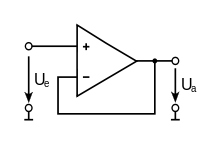
\includegraphics[scale=1]{bild/spannungsfolger}
\caption{Spannungsfolger Schaltung}
\end{center}
\end{figure}
\newpage
\subsection{Ergebnisse und Diskussion}
Tabelle 1 stellt die Ergebnisse der Offsetspannung dar. Auff\"allig ist, dass die Offsetspannung in dem Bereich U$_{dd}$ $\leq$ 4 sehr stark schwankt. \\
Zwischen $\pm$12~$V$ und $\pm$5~$V$ nimmt die Offsetspannung konstant leicht ab.\\ 
F\"ur U$_{\text{DD}}$ $=$ 2~$V$ ist die Offsetspannung sehr stark  negativ, hingegen steigt sie f\"ur U$_{\text{DD}}$ $=$ 1~$V$ auf 290,12~$mV$ an. Dies Verhalten l\"asst sich durch die Halbleitertechnik des Operationsverst\"arker erkl\"aren, dieser OPV besteht aus mehreren Transistoren, welche eine gewisse Spannung ben\"otigen, um den Strom leiten zu k\"onnen. 

\begin{table}[!ht]
\caption{Offsetspannung des Operationsverst\"arker}
\vspace{0.3cm}
\hspace{-1.2cm}
\begin{tabular}{|l|l|l|l|l|l|l|l|l|l|l|l|l|l|l|}
\hline
Betriebspannung & $\pm$0 & $\pm$ 1& $\pm$2& $\pm$3& $\pm$4& $\pm$5& $\pm$6 & $\pm$7& $\pm$8& $\pm$9& $\pm$10& $\pm$11 & $\pm$12 \\
U$_{\text{DD}}$ in $V$ & &&&&&&&&&&&& \\
\hline
Offsetspannung &4,40 & 290,12 & -50,28 & 1,68 & 2,22 & 2,36 & 2,46 & 2,54 & 2,63 & 2,66 & 2,71 & 2,77 & 2,82\\
U$_{\text{Off}}$ in $mV$ &&&&&&&&&&&&& \\
\hline
\end{tabular}
\end{table}